\documentclass[oneside]{book}\twocolumn
\usepackage[utf8]{inputenc}
\usepackage{pgfplots}
\pgfplotsset{compat=1.15}
\usepackage{mathrsfs}
\usetikzlibrary{arrows}
\usepackage{amsmath}
\usepackage{tikz}
\usepackage{wrapfig}
\usepackage{parskip}
\usepackage[most]{tcolorbox}
\usepackage{amssymb}
\usepackage{amsthm}
\usepackage[margin=0.7in]{geometry}
\usepackage{mathtools}
\usepackage{caption}
\usepackage{float}
\usepackage{enumitem}

\newtheorem{theorem}{Theorem}
\newtheorem{definition}[theorem]{Definition}
\newtheorem{claim}[theorem]{Claim}
\newtheorem{proposition}[theorem]{Proposition}
\newtheorem{lemma}[theorem]{Lemma}
\newtheorem{corollary}[theorem]{Corollary}
\newtheorem{conjecture}[theorem]{Conjecture}
\newtheorem*{observation}{Observation}
\newtheorem*{example}{Example}
\newtheorem*{remark}{Remark}

\usepackage{physics}
\usepackage{amsmath}
\usepackage{tikz}
\usepackage{mathdots}
\usepackage{yhmath}
\usepackage{cancel}
\usepackage{color}
\usepackage{siunitx}
\usepackage{array}
\usepackage{multirow}
\usepackage{amssymb}
\usepackage{gensymb}
\usepackage{tabularx}
\usepackage{extarrows}
\usepackage{booktabs}
\usetikzlibrary{fadings}
\usetikzlibrary{patterns}
\usetikzlibrary{shadows.blur}
\usetikzlibrary{shapes}




\tcbset{mytitle/.style={title={Question~\thetcbcounter\ifstrempty{#1}{}{: #1}}}}
\newtcolorbox[auto counter, number within=chapter, number freestyle={\noexpand\thechapter.\noexpand\arabic{\tcbcounter}}]{question}[1][]{%
    enhanced,
    breakable,
    fonttitle=\bfseries,
    mytitle={},
    #1
}


\title{Lecture Notes for Geometry of Curves and Surfaces\\ and \\the Riemann Uniformization Theorem}
\author{Aakash Ghosh }
\date{Instructor: Prof. Somnath Basu}
\begin{document}
\maketitle
\tableofcontents

\part{Course Notes}
\chapter{What to expect}
First we shall see some theorems and examples and get to know the terms on an intuitive sense. The formal definitions of everything will be provided down the line(probably).
\section{Four vertex theorem}
\begin{theorem}[Four Vertex Theorem]
The curvature of a simple closed smooth curve has at least 2 local minima and two local maxima.
\end{theorem}
\textbf{[Planar] Curve:} A curve is a map $f$ from $\mathbb R\to\mathbb R^2$. Note: other types of curves exists. For example, a space curve is a map from $\mathbb R\to\mathbb R^3$.\\
\textbf{Smooth:} Smooth implies that the $k^{th}$ derivative of $f$ defined in the previous section exists and is continuous for all $k\in\mathbb N$.\\
\textbf{Closed:} Intuitively, a closed curve has the same starting and ending point. We define $f:[0,c]\to\mathbb R^2$ as closed if $f(0)=f(c)$. If we want to define it according to the definition we gave earlier, we say $f$ is periodic. This implies for every $p\in\mathbb R$, $f(p+c)=f(p)$. The smallest such $c$ is known as the period of the function. We can also view this in an geometric way: A closed curve is a mapping of $S^1$ to $\mathbb R^2$($S^1$ is the unit circle in $\mathbb R^2$ plane). Let $e^{i\theta}$ be a point on $S^1$. Then a closed curve is a mapping $\Tilde{f}:S^1\to \mathbb{R}^2$. Now we can of course relate $\Tilde{f}$ and $f$ in a very natural way: $\Tilde{f}(e^{i\theta})=f(\frac{c}{2\pi}\theta)$(This result comes from the fact that the parameters which define $S^1$, i.e $\sin\theta$ and $\cos\theta$ are periodic in nature).\\
\textbf{Simple :}Intuitively, a simple curve is a curve which doesn't cross or touch itself. Therefore, if you zoom close enough at any point, it looks like a regular arc. mathematically we need $\Tilde{f}$ to be injective or one-one.


\tikzset{every picture/.style={line width=0.75pt}} %set default line width to 0.75pt        

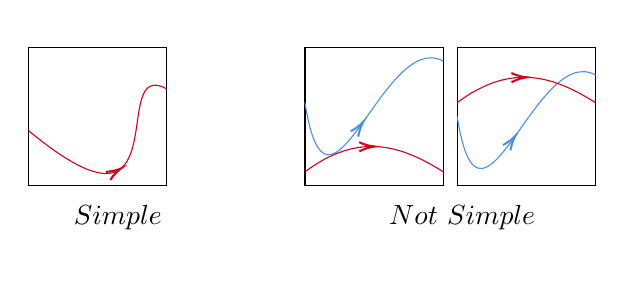
\begin{tikzpicture}[x=0.5pt,y=0.5pt,yscale=-1,xscale=1]
%uncomment if require: \path (0,300); %set diagram left start at 0, and has height of 300

%Shape: Rectangle [id:dp48033389218446143] 
\draw   (50,100) -- (150,100) -- (150,200) -- (50,200) -- cycle ;
%Shape: Rectangle [id:dp4215438801436513] 
\draw   (250,100) -- (350,100) -- (350,200) -- (250,200) -- cycle ;
%Shape: Rectangle [id:dp18460370937318105] 
\draw   (360,100) -- (460,100) -- (460,200) -- (360,200) -- cycle ;
%Curve Lines [id:da511310320695898] 
\draw [color={rgb, 255:red, 208; green, 2; blue, 27 }  ,draw opacity=1 ]   (50,160) .. controls (162.2,253) and (106.6,106.2) .. (150,130) ;
\draw [shift={(117.17,187.48)}, rotate = 150.29] [color={rgb, 255:red, 208; green, 2; blue, 27 }  ,draw opacity=1 ][line width=0.75]    (10.93,-3.29) .. controls (6.95,-1.4) and (3.31,-0.3) .. (0,0) .. controls (3.31,0.3) and (6.95,1.4) .. (10.93,3.29)   ;
%Curve Lines [id:da8342244921465348] 
\draw [color={rgb, 255:red, 74; green, 144; blue, 226 }  ,draw opacity=1 ]   (250,140) .. controls (267,248.2) and (306.6,86.2) .. (350,110) ;
\draw [shift={(292.21,153.72)}, rotate = 125.98] [color={rgb, 255:red, 74; green, 144; blue, 226 }  ,draw opacity=1 ][line width=0.75]    (10.93,-3.29) .. controls (6.95,-1.4) and (3.31,-0.3) .. (0,0) .. controls (3.31,0.3) and (6.95,1.4) .. (10.93,3.29)   ;
%Curve Lines [id:da35976819210964917] 
\draw [color={rgb, 255:red, 208; green, 2; blue, 27 }  ,draw opacity=1 ]   (250,190) .. controls (290,160) and (321,171.8) .. (350,190) ;
\draw [shift={(300.17,171.69)}, rotate = 178.96] [color={rgb, 255:red, 208; green, 2; blue, 27 }  ,draw opacity=1 ][line width=0.75]    (10.93,-3.29) .. controls (6.95,-1.4) and (3.31,-0.3) .. (0,0) .. controls (3.31,0.3) and (6.95,1.4) .. (10.93,3.29)   ;
%Curve Lines [id:da6101296278737137] 
\draw [color={rgb, 255:red, 74; green, 144; blue, 226 }  ,draw opacity=1 ]   (360,150) .. controls (377,258.2) and (416.6,96.2) .. (460,120) ;
\draw [shift={(402.21,163.72)}, rotate = 125.98] [color={rgb, 255:red, 74; green, 144; blue, 226 }  ,draw opacity=1 ][line width=0.75]    (10.93,-3.29) .. controls (6.95,-1.4) and (3.31,-0.3) .. (0,0) .. controls (3.31,0.3) and (6.95,1.4) .. (10.93,3.29)   ;
%Curve Lines [id:da6787942491941835] 
\draw [color={rgb, 255:red, 208; green, 2; blue, 27 }  ,draw opacity=1 ]   (360,140) .. controls (400,110) and (431,121.8) .. (460,140) ;
\draw [shift={(410.17,121.69)}, rotate = 178.96] [color={rgb, 255:red, 208; green, 2; blue, 27 }  ,draw opacity=1 ][line width=0.75]    (10.93,-3.29) .. controls (6.95,-1.4) and (3.31,-0.3) .. (0,0) .. controls (3.31,0.3) and (6.95,1.4) .. (10.93,3.29)   ;

% Text Node
\draw (81,212.4) node [anchor=north west][inner sep=0.75pt]    {$Simple$};
% Text Node
\draw (309,212.4) node [anchor=north west][inner sep=0.75pt]    {$Not\ Simple$};


\end{tikzpicture}

\textbf{Curvature :}Curvature is basically a function from the points of the curve to $\mathbb R$. Specifically $\mathcal{K}:\mathbb{R}^2\to\mathbb{R}$, where $\mathcal{K}(\Tilde{f}(e^{i\theta}))$ gives the inverse of the radius of the circle with the best fit at the point $\Tilde{f}(e^{i\theta})$. Now this circle of best fit needs to be defined with some care. for one the the point and the circle drawn share the same normal and tangent.
\begin{figure}[!htb]
    
\centering
\tikzset{every picture/.style={line width=0.75pt}} %set default line width to 0.75pt        

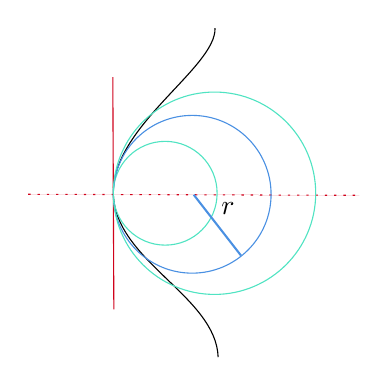
\begin{tikzpicture}[x=0.75pt,y=0.75pt,yscale=-1,xscale=1]
%uncomment if require: \path (0,300); %set diagram left start at 0, and has height of 300

%Curve Lines [id:da8990808912090099] 
\draw    (161,218.75) .. controls (160,189.25) and (111,172.25) .. (110.5,139.75) .. controls (110,107.25) and (160,79.25) .. (159.5,60.25) ;
%Straight Lines [id:da5329665639527169] 
\draw [color={rgb, 255:red, 208; green, 2; blue, 27 }  ,draw opacity=1 ]   (110.25,83.75) -- (110.75,195.75) ;
%Straight Lines [id:da996193084348262] 
\draw [color={rgb, 255:red, 208; green, 2; blue, 27 }  ,draw opacity=1 ][fill={rgb, 255:red, 208; green, 2; blue, 27 }  ,fill opacity=1 ] [dash pattern={on 0.84pt off 2.51pt}]  (69.5,140.25) -- (229,140.75) ;
%Shape: Circle [id:dp671885589792057] 
\draw  [color={rgb, 255:red, 80; green, 227; blue, 194 }  ,draw opacity=1 ] (110.5,139.75) .. controls (110.5,125.94) and (121.69,114.75) .. (135.5,114.75) .. controls (149.31,114.75) and (160.5,125.94) .. (160.5,139.75) .. controls (160.5,153.56) and (149.31,164.75) .. (135.5,164.75) .. controls (121.69,164.75) and (110.5,153.56) .. (110.5,139.75) -- cycle ;
%Shape: Circle [id:dp916983786523555] 
\draw  [color={rgb, 255:red, 74; green, 144; blue, 226 }  ,draw opacity=1 ] (110.5,140.25) .. controls (110.5,119.26) and (127.51,102.25) .. (148.5,102.25) .. controls (169.49,102.25) and (186.5,119.26) .. (186.5,140.25) .. controls (186.5,161.24) and (169.49,178.25) .. (148.5,178.25) .. controls (127.51,178.25) and (110.5,161.24) .. (110.5,140.25) -- cycle ;
%Shape: Circle [id:dp7636897615627564] 
\draw  [color={rgb, 255:red, 80; green, 227; blue, 194 }  ,draw opacity=1 ] (110.5,139.75) .. controls (110.5,112.83) and (132.33,91) .. (159.25,91) .. controls (186.17,91) and (208,112.83) .. (208,139.75) .. controls (208,166.67) and (186.17,188.5) .. (159.25,188.5) .. controls (132.33,188.5) and (110.5,166.67) .. (110.5,139.75) -- cycle ;
%Straight Lines [id:da3292244417302711] 
\draw [color={rgb, 255:red, 74; green, 144; blue, 226 }  ,draw opacity=1 ][line width=0.75]    (149.25,140.5) -- (172,169.75) ;

% Text Node
\draw (161.25,143.15) node [anchor=north west][inner sep=0.75pt]    {$r$};


\end{tikzpicture}

    \caption{The red lines are common normal and common tangent. Note, the circle of medium size somehow seems to be a better fit than the others. So the radius of curvature at that point is $\frac{1}{r}$}
    \label{fig:my_label}
\end{figure}
One way to drive this concept home for planar curve is to consider the following process: take any three points $t_1,t_2,t_3$ around $t$. Draw the circumcircle of those points. the radius of curvature will be the radius of the circle formed when $\lim{t_1,t_2,t_3\to t}$


\tikzset{every picture/.style={line width=0.75pt}} %set default line width to 0.75pt        

\begin{tikzpicture}[x=0.75pt,y=0.75pt,yscale=-1,xscale=1]
%uncomment if require: \path (0,300); %set diagram left start at 0, and has height of 300

%Curve Lines [id:da026905970078967] 
\draw    (51.43,191.95) .. controls (224.17,191.05) and (197.6,149.86) .. (219.84,149.86) .. controls (242.09,149.86) and (222.32,191.05) .. (417,192.24) ;
%Shape: Ellipse [id:dp8371132730905899] 
\draw  [color={rgb, 255:red, 208; green, 2; blue, 27 }  ,draw opacity=1 ] (176.89,208.36) .. controls (176.89,179.51) and (201.1,156.13) .. (230.97,156.13) .. controls (260.84,156.13) and (285.05,179.51) .. (285.05,208.36) .. controls (285.05,237.21) and (260.84,260.6) .. (230.97,260.6) .. controls (201.1,260.6) and (176.89,237.21) .. (176.89,208.36) -- cycle ;

% Text Node
\draw (175.66,150.49) node [anchor=north west][inner sep=0.75pt]    {$t_{1}$};
% Text Node
\draw (232.86,135.29) node [anchor=north west][inner sep=0.75pt]    {$t_{2}$};
% Text Node
\draw (276.46,158.49) node [anchor=north west][inner sep=0.75pt]    {$t_{3}$};
% Text Node
\draw (214,131.6) node [anchor=north west][inner sep=0.75pt]    {$t$};


\end{tikzpicture}
The figure above shows the process. While this is nice way to view things, it is has it's own set of problems: How do we know that a limit exists? More over in higher dimensional spaces, the plane in which the circle lies will also change with the points that are being considered. Nevertheless it's good enough for a naive mental picture. The rest of the theorem now makes sense. 














\section{Fary-Milnor theorem}
\begin{theorem}[Fary-Milnor theorem]
If the total absolute curvature of a knot $K$ is at most $4\pi$, then $K$ is an unknot.
\end{theorem}
\textbf{Knot :}A knot is a simple curve in 3-space. 
\textbf{Total absolute curvature :}What it says. We can't of course take an infinite sum for all the points so we integrate. 
\begin{align}
    S=\int_\mathcal{S}\left|\mathcal{K}(s)\right|ds
\end{align}
\textbf{Unknot :}A unknot is a knot which can be deformed to a circle.
\begin{figure}[!htb]
    \centering
    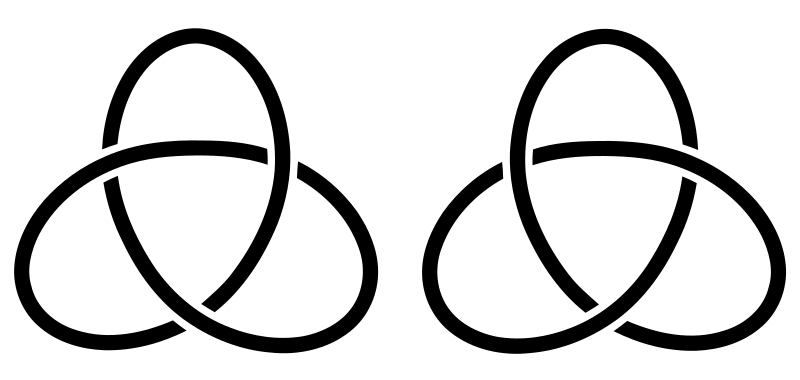
\includegraphics[width=0.45\textwidth]{The_two_trefoil_knots.png}
    \caption{The two trefoil knots. They are not unknots(Copied from Wikipedia)}
    \label{fig:my_label}
\end{figure}
\section{Hirsch-Smale Theory}
\begin{theorem}[Hirsch-Smale Theory]
Any two immersed loop in $\mathbb R^2$ are isotopic if and only if the winding numbers match.
\end{theorem}
\textbf{Loop:} A loop is a closed curve\\
\textbf{Immersed:} $f:\mathbb R\to\mathbb R^k$ is said to be immersed if $f'(t)$ is never zero. Note, the drawing of any curve is the trace of a curve: It does not represent the curve itself.\\
\textbf{Isotopic:} This means they are the same. It is what isomorphism is for groups and homeomorphism is for topologies. But when are two loops isotopic?
\begin{figure}[!htb]
    \centering
    

\tikzset{every picture/.style={line width=0.75pt}} %set default line width to 0.75pt        

\begin{tikzpicture}[x=0.5pt,y=0.5pt,yscale=-1,xscale=1]
%uncomment if require: \path (0,300); %set diagram left start at 0, and has height of 300

%Shape: Circle [id:dp3439595731687489] 
\draw   (20,100) .. controls (20,55.82) and (55.82,20) .. (100,20) .. controls (144.18,20) and (180,55.82) .. (180,100) .. controls (180,144.18) and (144.18,180) .. (100,180) .. controls (55.82,180) and (20,144.18) .. (20,100) -- cycle ;
%Shape: Triangle [id:dp1382493260916383] 
\draw  [fill={rgb, 255:red, 0; green, 0; blue, 0 }  ,fill opacity=1 ] (135.32,28.16) -- (126,28.81) -- (132.5,19.25) -- cycle ;
%Curve Lines [id:da9272590436110197] 
\draw    (236,40.5) .. controls (276,10.5) and (368,-0.25) .. (336,40.5) .. controls (304,81.25) and (454,85.25) .. (375.5,140.25) .. controls (297,195.25) and (180,204.25) .. (255,121.25) .. controls (330,38.25) and (211,65.5) .. (236,40.5) -- cycle ;
\draw [shift={(298.5,15.66)}, rotate = 169.09] [fill={rgb, 255:red, 0; green, 0; blue, 0 }  ][line width=0.08]  [draw opacity=0] (8.93,-4.29) -- (0,0) -- (8.93,4.29) -- cycle    ;
\draw [shift={(377.38,87.39)}, rotate = 209.14] [fill={rgb, 255:red, 0; green, 0; blue, 0 }  ][line width=0.08]  [draw opacity=0] (8.93,-4.29) -- (0,0) -- (8.93,4.29) -- cycle    ;
\draw [shift={(277.57,181.23)}, rotate = 350.42] [fill={rgb, 255:red, 0; green, 0; blue, 0 }  ][line width=0.08]  [draw opacity=0] (8.93,-4.29) -- (0,0) -- (8.93,4.29) -- cycle    ;
\draw [shift={(278.02,69.26)}, rotate = 70.96] [fill={rgb, 255:red, 0; green, 0; blue, 0 }  ][line width=0.08]  [draw opacity=0] (8.93,-4.29) -- (0,0) -- (8.93,4.29) -- cycle    ;

% Text Node
\draw (93,212.4) node [anchor=north west][inner sep=0.75pt]    {$\gamma $};
% Text Node
\draw (308.5,210.9) node [anchor=north west][inner sep=0.75pt]    {$\eta $};


\end{tikzpicture}



    \caption{Two isotopic curves: The second one can be "straightened out" into the first one}
    \label{fig:my_label}
\end{figure}
But how to check this? We construct a $f$ which deforms $\eta$ to $\gamma$. But note: merely the presence of such a function is not enough. This would imply any two loops are isotopic. We furthermore require at any instant of the transformation, the resulting curve is  immersed. Now we shall talk a bit about the function. Let $H:S^1\times I\to\mathbb R^2$, where $I=[0,1]$. Now note that the set $S^1\times I\to\mathbb R^2$ looks like a cylinder. $S^1$ represents the base, $I$ represents the height. We think of moving along $I$ as moving along time. The base of the cylinder is the curve when we start(i.e. $H(S^1\times\{0\})$) and the top of the cylinder is the curve we end up with(i.e. $H(S^1\times\{1\})$). We also need $H(S^1\times t)$ to be immersed.\\
\begin{figure}[!htb]
    \centering
    

\tikzset{every picture/.style={line width=0.75pt}} %set default line width to 0.75pt        

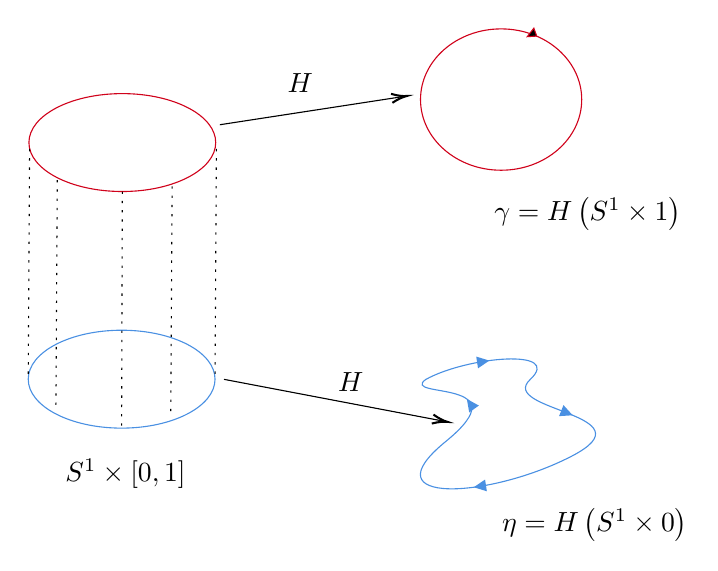
\begin{tikzpicture}[x=0.5pt,y=0.5pt,yscale=-1,xscale=1]
%uncomment if require: \path (0,414); %set diagram left start at 0, and has height of 414

%Shape: Ellipse [id:dp8580791830403575] 
\draw  [color={rgb, 255:red, 208; green, 2; blue, 27 }  ,draw opacity=1 ] (344.5,83.8) .. controls (344.5,55.59) and (370.58,32.73) .. (402.75,32.73) .. controls (434.92,32.73) and (461,55.59) .. (461,83.8) .. controls (461,112) and (434.92,134.87) .. (402.75,134.87) .. controls (370.58,134.87) and (344.5,112) .. (344.5,83.8) -- cycle ;
%Shape: Triangle [id:dp1741505392127638] 
\draw  [color={rgb, 255:red, 208; green, 2; blue, 27 }  ,draw opacity=1 ][fill={rgb, 255:red, 0; green, 0; blue, 0 }  ,fill opacity=1 ] (428.46,37.93) -- (421.68,38.35) -- (426.41,32.25) -- cycle ;

%Curve Lines [id:da2246700601326841] 
\draw [color={rgb, 255:red, 74; green, 144; blue, 226 }  ,draw opacity=1 ]   (348.25,286.09) .. controls (378.46,269.4) and (447.94,263.42) .. (423.78,286.09) .. controls (399.61,308.76) and (512.89,310.99) .. (453.61,341.59) .. controls (394.32,372.19) and (305.96,377.19) .. (362.6,331.02) .. controls (419.25,284.84) and (329.37,300) .. (348.25,286.09) -- cycle ;
\draw [shift={(394.24,272.44)}, rotate = 171.27] [fill={rgb, 255:red, 74; green, 144; blue, 226 }  ,fill opacity=1 ][line width=0.08]  [draw opacity=0] (8.93,-4.29) -- (0,0) -- (8.93,4.29) -- cycle    ;
\draw [shift={(454.51,311.96)}, rotate = 201.95] [fill={rgb, 255:red, 74; green, 144; blue, 226 }  ,fill opacity=1 ][line width=0.08]  [draw opacity=0] (8.93,-4.29) -- (0,0) -- (8.93,4.29) -- cycle    ;
\draw [shift={(382.98,363.98)}, rotate = 351.41] [fill={rgb, 255:red, 74; green, 144; blue, 226 }  ,fill opacity=1 ][line width=0.08]  [draw opacity=0] (8.93,-4.29) -- (0,0) -- (8.93,4.29) -- cycle    ;
\draw [shift={(377.98,300.18)}, rotate = 54.37] [fill={rgb, 255:red, 74; green, 144; blue, 226 }  ,fill opacity=1 ][line width=0.08]  [draw opacity=0] (8.93,-4.29) -- (0,0) -- (8.93,4.29) -- cycle    ;

%Shape: Ellipse [id:dp5051354795111995] 
\draw  [color={rgb, 255:red, 208; green, 2; blue, 27 }  ,draw opacity=1 ] (61.5,114.88) .. controls (61.5,95.34) and (91.72,79.5) .. (129,79.5) .. controls (166.28,79.5) and (196.5,95.34) .. (196.5,114.88) .. controls (196.5,134.41) and (166.28,150.25) .. (129,150.25) .. controls (91.72,150.25) and (61.5,134.41) .. (61.5,114.88) -- cycle ;
%Shape: Ellipse [id:dp028752110313813417] 
\draw  [color={rgb, 255:red, 74; green, 144; blue, 226 }  ,draw opacity=1 ] (61,285.88) .. controls (61,266.34) and (91.22,250.5) .. (128.5,250.5) .. controls (165.78,250.5) and (196,266.34) .. (196,285.88) .. controls (196,305.41) and (165.78,321.25) .. (128.5,321.25) .. controls (91.22,321.25) and (61,305.41) .. (61,285.88) -- cycle ;
%Straight Lines [id:da6715965743533834] 
\draw  [dash pattern={on 0.84pt off 2.51pt}]  (62,119.5) -- (61,285.88) ;
%Straight Lines [id:da24973361821393547] 
\draw  [dash pattern={on 0.84pt off 2.51pt}]  (82,142) -- (81,308.38) ;
%Straight Lines [id:da664998350332383] 
\draw  [dash pattern={on 0.84pt off 2.51pt}]  (129,150.25) -- (128.5,321.25) ;
%Straight Lines [id:da0662385964287534] 
\draw  [dash pattern={on 0.84pt off 2.51pt}]  (165,146.5) -- (164,312.88) ;
%Straight Lines [id:da3891917682172963] 
\draw  [dash pattern={on 0.84pt off 2.51pt}]  (197,119.5) -- (196,285.88) ;
%Straight Lines [id:da7252691499439365] 
\draw    (199.5,102) -- (332.52,81.55) ;
\draw [shift={(334.5,81.25)}, rotate = 171.26] [color={rgb, 255:red, 0; green, 0; blue, 0 }  ][line width=0.75]    (10.93,-3.29) .. controls (6.95,-1.4) and (3.31,-0.3) .. (0,0) .. controls (3.31,0.3) and (6.95,1.4) .. (10.93,3.29)   ;
%Straight Lines [id:da7874706184444381] 
\draw    (202.5,286) -- (362.04,316.38) ;
\draw [shift={(364,316.75)}, rotate = 190.78] [color={rgb, 255:red, 0; green, 0; blue, 0 }  ][line width=0.75]    (10.93,-3.29) .. controls (6.95,-1.4) and (3.31,-0.3) .. (0,0) .. controls (3.31,0.3) and (6.95,1.4) .. (10.93,3.29)   ;

% Text Node
\draw (401.54,377.52) node [anchor=north west][inner sep=0.75pt]    {$\eta =H\left( S^{1} \times 0\right)$};
% Text Node
\draw (396.02,152.8) node [anchor=north west][inner sep=0.75pt]    {$\gamma =H\left( S^{1} \times 1\right)$};
% Text Node
\draw (246.5,63.4) node [anchor=north west][inner sep=0.75pt]    {$H$};
% Text Node
\draw (283,278.9) node [anchor=north west][inner sep=0.75pt]    {$H$};
% Text Node
\draw (86,341.9) node [anchor=north west][inner sep=0.75pt]    {$S^{1} \times [ 0,1]$};


\end{tikzpicture}

    \caption{Representation of $H$}
    \label{fig:my_label}
\end{figure}
\textbf{Winding number: }It is the total number of loops we make when we complete traversing closed curve. Alternatively, imagine holding out a compass needle. Then the total number of complete turns the needle makes will be the winding number.
\begin{figure}[!htb]
    \centering
    

\tikzset{every picture/.style={line width=0.75pt}} %set default line width to 0.75pt        

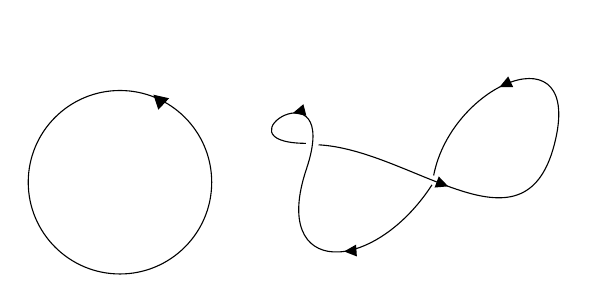
\begin{tikzpicture}[x=0.5pt,y=0.5pt,yscale=-1,xscale=1]
%uncomment if require: \path (0,300); %set diagram left start at 0, and has height of 300

%Shape: Circle [id:dp9595274264781469] 
\draw   (40,105.9) .. controls (40,69.28) and (69.68,39.6) .. (106.3,39.6) .. controls (142.92,39.6) and (172.6,69.28) .. (172.6,105.9) .. controls (172.6,142.52) and (142.92,172.2) .. (106.3,172.2) .. controls (69.68,172.2) and (40,142.52) .. (40,105.9) -- cycle ;
%Curve Lines [id:da6184433689903426] 
\draw    (240.6,77.8) .. controls (173,77.4) and (267.4,17.8) .. (240.99,96.55) .. controls (214.59,175.31) and (289.21,173.29) .. (331.8,107.8) ;
\draw [shift={(231.29,55.9)}, rotate = 345.54] [fill={rgb, 255:red, 0; green, 0; blue, 0 }  ][line width=0.08]  [draw opacity=0] (8.93,-4.29) -- (0,0) -- (8.93,4.29) -- cycle    ;
\draw [shift={(268.31,155.91)}, rotate = 355.98] [fill={rgb, 255:red, 0; green, 0; blue, 0 }  ][line width=0.08]  [draw opacity=0] (8.93,-4.29) -- (0,0) -- (8.93,4.29) -- cycle    ;
%Curve Lines [id:da37718589291443505] 
\draw    (249.79,78.86) .. controls (317.6,82.53) and (398.11,163.13) .. (420.15,78.86) .. controls (442.2,-5.4) and (345.95,33.94) .. (333,101) ;
\draw [shift={(343.53,108.87)}, rotate = 200.62] [fill={rgb, 255:red, 0; green, 0; blue, 0 }  ][line width=0.08]  [draw opacity=0] (8.93,-4.29) -- (0,0) -- (8.93,4.29) -- cycle    ;
\draw [shift={(380.59,37.11)}, rotate = 334.94] [fill={rgb, 255:red, 0; green, 0; blue, 0 }  ][line width=0.08]  [draw opacity=0] (8.93,-4.29) -- (0,0) -- (8.93,4.29) -- cycle    ;
%Shape: Triangle [id:dp8787590147736832] 
\draw  [fill={rgb, 255:red, 0; green, 0; blue, 0 }  ,fill opacity=1 ] (134.18,52.72) -- (131.09,43.21) -- (141.04,45.45) -- cycle ;




\end{tikzpicture}

    \caption{Winding number 1}
    \label{fig:my_label}
\end{figure}

\begin{figure}[!htb]
    \centering
    

\tikzset{every picture/.style={line width=0.75pt}} %set default line width to 0.75pt        

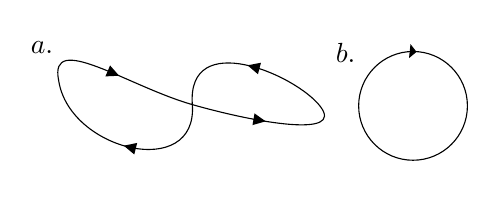
\begin{tikzpicture}[x=0.5pt,y=0.5pt,yscale=-1,xscale=1]
%uncomment if require: \path (0,300); %set diagram left start at 0, and has height of 300

%Curve Lines [id:da2718429255912467] 
\draw    (43.6,41.2) .. controls (36.2,5) and (93.8,45.4) .. (140.2,58.6) .. controls (186.6,71.8) and (250.6,83) .. (232.6,59.8) .. controls (214.6,36.6) and (136.2,3.4) .. (140.2,58.6) .. controls (144.2,113.8) and (51.4,92.2) .. (43.6,41.2) -- cycle ;
\draw [shift={(87.29,37.75)}, rotate = 203.05] [fill={rgb, 255:red, 0; green, 0; blue, 0 }  ][line width=0.08]  [draw opacity=0] (8.93,-4.29) -- (0,0) -- (8.93,4.29) -- cycle    ;
\draw [shift={(193.2,70.68)}, rotate = 189.74] [fill={rgb, 255:red, 0; green, 0; blue, 0 }  ][line width=0.08]  [draw opacity=0] (8.93,-4.29) -- (0,0) -- (8.93,4.29) -- cycle    ;
\draw [shift={(180.08,30.21)}, rotate = 14.73] [fill={rgb, 255:red, 0; green, 0; blue, 0 }  ][line width=0.08]  [draw opacity=0] (8.93,-4.29) -- (0,0) -- (8.93,4.29) -- cycle    ;
\draw [shift={(90.63,88.3)}, rotate = 14.01] [fill={rgb, 255:red, 0; green, 0; blue, 0 }  ][line width=0.08]  [draw opacity=0] (8.93,-4.29) -- (0,0) -- (8.93,4.29) -- cycle    ;
%Shape: Circle [id:dp8907209896109666] 
\draw   (260.4,59.5) .. controls (260.4,37.8) and (278,20.2) .. (299.7,20.2) .. controls (321.4,20.2) and (339,37.8) .. (339,59.5) .. controls (339,81.2) and (321.4,98.8) .. (299.7,98.8) .. controls (278,98.8) and (260.4,81.2) .. (260.4,59.5) -- cycle ;
%Shape: Triangle [id:dp6641882002067809] 
\draw  [fill={rgb, 255:red, 0; green, 0; blue, 0 }  ,fill opacity=1 ] (301.69,20.41) -- (297.29,24.07) -- (298.14,15.91) -- cycle ;

% Text Node
\draw (21.6,11.2) node [anchor=north west][inner sep=0.75pt]    {$a.$};
% Text Node
\draw (242,12.6) node [anchor=north west][inner sep=0.75pt]    {$b.$};


\end{tikzpicture}

    \caption{a. Winding number 0 b. Winding number -1}
    \label{fig:my_label}
\end{figure}

But what if we consider curves in $S^2$? Then the theorem changes as follows:

\begin{theorem}[Hirsch-Smale Theory, $2^{nd}$ part]
Any two immersed loop in $S^2$ are isotopic if and only if the winding numbers match modulo 2.
\end{theorem}
\begin{figure*}[!htb]
    \centering
    

% Gradient Info
  
\tikzset {_o50ed9ycy/.code = {\pgfsetadditionalshadetransform{ \pgftransformshift{\pgfpoint{0 bp } { 0 bp }  }  \pgftransformscale{1 }  }}}
\pgfdeclareradialshading{_gk5204urd}{\pgfpoint{0bp}{0bp}}{rgb(0bp)=(1,1,1);
rgb(0bp)=(1,1,1);
rgb(25bp)=(0.29,0.56,0.89);
rgb(400bp)=(0.29,0.56,0.89)}

% Gradient Info
  
\tikzset {_2m37d3yfb/.code = {\pgfsetadditionalshadetransform{ \pgftransformshift{\pgfpoint{0 bp } { 0 bp }  }  \pgftransformscale{1 }  }}}
\pgfdeclareradialshading{_6smwnwe06}{\pgfpoint{0bp}{0bp}}{rgb(0bp)=(1,1,1);
rgb(0bp)=(1,1,1);
rgb(25bp)=(0.29,0.56,0.89);
rgb(400bp)=(0.29,0.56,0.89)}

% Gradient Info
  
\tikzset {_b6wkzg2sw/.code = {\pgfsetadditionalshadetransform{ \pgftransformshift{\pgfpoint{0 bp } { 0 bp }  }  \pgftransformscale{1 }  }}}
\pgfdeclareradialshading{_s15twwqz4}{\pgfpoint{0bp}{0bp}}{rgb(0bp)=(1,1,1);
rgb(0bp)=(1,1,1);
rgb(25bp)=(0.29,0.56,0.89);
rgb(400bp)=(0.29,0.56,0.89)}
\tikzset{every picture/.style={line width=0.75pt}} %set default line width to 0.75pt        

\begin{tikzpicture}[x=0.75pt,y=0.75pt,yscale=-1,xscale=1]
%uncomment if require: \path (0,300); %set diagram left start at 0, and has height of 300

%Shape: Circle [id:dp4428149399613551] 
\path  [shading=_gk5204urd,_o50ed9ycy] (40.8,131.5) .. controls (40.8,86.82) and (77.02,50.6) .. (121.7,50.6) .. controls (166.38,50.6) and (202.6,86.82) .. (202.6,131.5) .. controls (202.6,176.18) and (166.38,212.4) .. (121.7,212.4) .. controls (77.02,212.4) and (40.8,176.18) .. (40.8,131.5) -- cycle ; % for fading 
 \draw  [color={rgb, 255:red, 74; green, 144; blue, 226 }  ,draw opacity=1 ] (40.8,131.5) .. controls (40.8,86.82) and (77.02,50.6) .. (121.7,50.6) .. controls (166.38,50.6) and (202.6,86.82) .. (202.6,131.5) .. controls (202.6,176.18) and (166.38,212.4) .. (121.7,212.4) .. controls (77.02,212.4) and (40.8,176.18) .. (40.8,131.5) -- cycle ; % for border 

%Shape: Circle [id:dp10055389125205716] 
\draw  [color={rgb, 255:red, 208; green, 2; blue, 27 }  ,draw opacity=1 ] (81.6,131.5) .. controls (81.6,109.35) and (99.55,91.4) .. (121.7,91.4) .. controls (143.85,91.4) and (161.8,109.35) .. (161.8,131.5) .. controls (161.8,153.65) and (143.85,171.6) .. (121.7,171.6) .. controls (99.55,171.6) and (81.6,153.65) .. (81.6,131.5) -- cycle ;
%Shape: Triangle [id:dp3509374145983808] 
\draw  [fill={rgb, 255:red, 0; green, 0; blue, 0 }  ,fill opacity=1 ] (125,91.5) -- (118.29,95) -- (118.51,87.61) -- cycle ;
%Straight Lines [id:da5671120603581383] 
\draw    (210.8,119.6) -- (274.2,120.57) ;
\draw [shift={(276.2,120.6)}, rotate = 180.88] [color={rgb, 255:red, 0; green, 0; blue, 0 }  ][line width=0.75]    (10.93,-3.29) .. controls (6.95,-1.4) and (3.31,-0.3) .. (0,0) .. controls (3.31,0.3) and (6.95,1.4) .. (10.93,3.29)   ;
%Curve Lines [id:da8668609867265892] 
\draw  [dash pattern={on 4.5pt off 4.5pt}]  (156.8,100.4) .. controls (156.21,59.25) and (175.97,39.21) .. (196.98,53.44) ;
\draw [shift={(198.6,54.6)}, rotate = 217.21] [color={rgb, 255:red, 0; green, 0; blue, 0 }  ][line width=0.75]    (10.93,-3.29) .. controls (6.95,-1.4) and (3.31,-0.3) .. (0,0) .. controls (3.31,0.3) and (6.95,1.4) .. (10.93,3.29)   ;
%Curve Lines [id:da49265357313711355] 
\draw  [dash pattern={on 4.5pt off 4.5pt}]  (80.8,100.4) .. controls (80.21,58.83) and (73.99,27.55) .. (51.25,57.2) ;
\draw [shift={(50.2,58.6)}, rotate = 306.41] [color={rgb, 255:red, 0; green, 0; blue, 0 }  ][line width=0.75]    (10.93,-3.29) .. controls (6.95,-1.4) and (3.31,-0.3) .. (0,0) .. controls (3.31,0.3) and (6.95,1.4) .. (10.93,3.29)   ;
%Curve Lines [id:da05561541607024678] 
\draw  [dash pattern={on 4.5pt off 4.5pt}]  (160,168.8) .. controls (159.8,219.56) and (238.94,217.51) .. (222.9,191.43) ;
\draw [shift={(221.8,189.8)}, rotate = 53.53] [color={rgb, 255:red, 0; green, 0; blue, 0 }  ][line width=0.75]    (10.93,-3.29) .. controls (6.95,-1.4) and (3.31,-0.3) .. (0,0) .. controls (3.31,0.3) and (6.95,1.4) .. (10.93,3.29)   ;
%Curve Lines [id:da23945267738357534] 
\draw  [dash pattern={on 4.5pt off 4.5pt}]  (88.4,169.6) .. controls (88.2,220.88) and (36.84,239.04) .. (41.64,193.21) ;
\draw [shift={(41.8,191.8)}, rotate = 97.18] [color={rgb, 255:red, 0; green, 0; blue, 0 }  ][line width=0.75]    (10.93,-3.29) .. controls (6.95,-1.4) and (3.31,-0.3) .. (0,0) .. controls (3.31,0.3) and (6.95,1.4) .. (10.93,3.29)   ;
%Shape: Circle [id:dp8287841133971156] 
\path  [shading=_6smwnwe06,_2m37d3yfb] (286.8,122.7) .. controls (286.8,78.02) and (323.02,41.8) .. (367.7,41.8) .. controls (412.38,41.8) and (448.6,78.02) .. (448.6,122.7) .. controls (448.6,167.38) and (412.38,203.6) .. (367.7,203.6) .. controls (323.02,203.6) and (286.8,167.38) .. (286.8,122.7) -- cycle ; % for fading 
 \draw  [color={rgb, 255:red, 74; green, 144; blue, 226 }  ,draw opacity=1 ] (286.8,122.7) .. controls (286.8,78.02) and (323.02,41.8) .. (367.7,41.8) .. controls (412.38,41.8) and (448.6,78.02) .. (448.6,122.7) .. controls (448.6,167.38) and (412.38,203.6) .. (367.7,203.6) .. controls (323.02,203.6) and (286.8,167.38) .. (286.8,122.7) -- cycle ; % for border 

%Shape: Circle [id:dp3582440477404123] 
\draw  [color={rgb, 255:red, 208; green, 2; blue, 27 }  ,draw opacity=1 ][dash pattern={on 4.5pt off 4.5pt}] (327.6,122.7) .. controls (327.6,100.55) and (345.55,82.6) .. (367.7,82.6) .. controls (389.85,82.6) and (407.8,100.55) .. (407.8,122.7) .. controls (407.8,144.85) and (389.85,162.8) .. (367.7,162.8) .. controls (345.55,162.8) and (327.6,144.85) .. (327.6,122.7) -- cycle ;
%Shape: Triangle [id:dp57592370617849] 
\draw  [fill={rgb, 255:red, 0; green, 0; blue, 0 }  ,fill opacity=1 ] (354.35,85.34) -- (349.67,91.28) -- (346.84,84.44) -- cycle ;
%Straight Lines [id:da6906001583873703] 
\draw    (368.2,19.8) -- (367.2,225.6) ;
%Curve Lines [id:da47646965878996683] 
\draw    (350.2,31) .. controls (300.81,50.21) and (434.28,50.21) .. (394.83,31) ;
\draw [shift={(392.2,29.8)}, rotate = 23.2] [fill={rgb, 255:red, 0; green, 0; blue, 0 }  ][line width=0.08]  [draw opacity=0] (8.93,-4.29) -- (0,0) -- (8.93,4.29) -- cycle    ;
%Shape: Circle [id:dp6404134705913701] 
\path  [shading=_s15twwqz4,_b6wkzg2sw] (522.8,119.1) .. controls (522.8,74.42) and (559.02,38.2) .. (603.7,38.2) .. controls (648.38,38.2) and (684.6,74.42) .. (684.6,119.1) .. controls (684.6,163.78) and (648.38,200) .. (603.7,200) .. controls (559.02,200) and (522.8,163.78) .. (522.8,119.1) -- cycle ; % for fading 
 \draw  [color={rgb, 255:red, 74; green, 144; blue, 226 }  ,draw opacity=1 ] (522.8,119.1) .. controls (522.8,74.42) and (559.02,38.2) .. (603.7,38.2) .. controls (648.38,38.2) and (684.6,74.42) .. (684.6,119.1) .. controls (684.6,163.78) and (648.38,200) .. (603.7,200) .. controls (559.02,200) and (522.8,163.78) .. (522.8,119.1) -- cycle ; % for border 

%Shape: Circle [id:dp020289716418068426] 
\draw  [color={rgb, 255:red, 208; green, 2; blue, 27 }  ,draw opacity=1 ] (563.6,119.1) .. controls (563.6,96.95) and (581.55,79) .. (603.7,79) .. controls (625.85,79) and (643.8,96.95) .. (643.8,119.1) .. controls (643.8,141.25) and (625.85,159.2) .. (603.7,159.2) .. controls (581.55,159.2) and (563.6,141.25) .. (563.6,119.1) -- cycle ;
%Shape: Triangle [id:dp8243051535367023] 
\draw  [fill={rgb, 255:red, 0; green, 0; blue, 0 }  ,fill opacity=1 ] (600.4,79.05) -- (606.94,75.25) -- (607.05,82.65) -- cycle ;
%Straight Lines [id:da5989560347824799] 
\draw    (452.4,119.2) -- (515.8,120.17) ;
\draw [shift={(517.8,120.2)}, rotate = 180.88] [color={rgb, 255:red, 0; green, 0; blue, 0 }  ][line width=0.75]    (10.93,-3.29) .. controls (6.95,-1.4) and (3.31,-0.3) .. (0,0) .. controls (3.31,0.3) and (6.95,1.4) .. (10.93,3.29)   ;




\end{tikzpicture}

    \caption{Example of part two of theorem. The winding number changes from -1 to +1. The dotted lines represent the curve on the rear side of the sphere.}
    \label{fig:my_label}
\end{figure*}

\chapter{Curves}
\section{Introduction}
We shall first consider some probable definitions of curves and see why they are wrong.
\begin{enumerate}
    \item \textbf{A curve is a set with empty interior}. This on the first glance looks pretty good: after all our by our geometric intuition, a curve has nothing inside it. But while it does take into account all things we intuitively understand as curve, there are things included in this which are not very curve like. For example, consider:
    $$f(x,y)=\begin{cases}1\quad&x\in\mathbb Q\times\mathbb Q\\ 0\quad&x\notin\mathbb Q\times\mathbb Q\end{cases}$$
    As $\mathbb Q$ is dense in $\mathbb R$, $S=\{(x,y)|f(x,y)=0\}$ has a empty interior. But it's obvious that $S$ which has some weird appearance is definitely not a curve.
  \item\textbf{A curve is the graph of a function.} Therefore, every curve can be represented as $(x,f(x))$ or $(x,f_1(x),f_2(x))$. This definition suffers from the opposite problem of the previous definition. Note, structures like a vertical line($y=k$) or a parabola($x=y^2$) can not be graphs of functions because they fail the vertical line test and are yet curves.
  \begin{figure}[H]
      \centering
      

\tikzset{every picture/.style={line width=0.75pt}} %set default line width to 0.75pt        

\begin{tikzpicture}[x=0.75pt,y=0.75pt,yscale=-1,xscale=1]
%uncomment if require: \path (0,300); %set diagram left start at 0, and has height of 300

%Curve Lines [id:da21071482613616144] 
\draw    (32.33,14.17) .. controls (78,15.5) and (-23.67,80.83) .. (39,55.83) .. controls (101.67,30.83) and (-2.67,105.5) .. (38,113.17) ;
%Shape: Arc [id:dp004048976867261689] 
\draw  [draw opacity=0] (155.45,96.51) .. controls (151.7,96.94) and (147.81,97.17) .. (143.83,97.17) .. controls (111.89,97.17) and (86,82.58) .. (86,64.58) .. controls (86,46.59) and (111.89,32) .. (143.83,32) .. controls (162.24,32) and (178.63,36.84) .. (189.23,44.39) -- (143.83,64.58) -- cycle ; \draw   (155.45,96.51) .. controls (151.7,96.94) and (147.81,97.17) .. (143.83,97.17) .. controls (111.89,97.17) and (86,82.58) .. (86,64.58) .. controls (86,46.59) and (111.89,32) .. (143.83,32) .. controls (162.24,32) and (178.63,36.84) .. (189.23,44.39) ;
%Straight Lines [id:da4986095954483222] 
\draw  [dash pattern={on 0.84pt off 2.51pt}]  (39,7.33) -- (38.33,118.17) ;
%Straight Lines [id:da8847804148280588] 
\draw  [dash pattern={on 0.84pt off 2.51pt}]  (120,8.33) -- (120,117.5) ;




\end{tikzpicture}

      \caption{Two curves which are not graphs of a function}
      \label{fig:my_label}
  \end{figure}
  \item\textbf{A curve is the set of points where a function vanishes.} We might think this works: after all, we can now circumnavigate around our previous problem by making an suitable function like $f(x,y):=y-k$ or $f(x,y):=x-y^2$. But this again makes things which are intuitively not a curve, a curve.
  \begin{figure}[H]
      \centering
      

\tikzset{every picture/.style={line width=0.75pt}} %set default line width to 0.75pt        

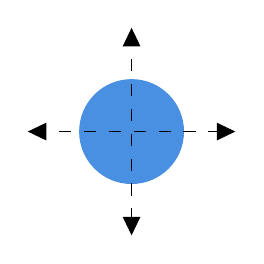
\begin{tikzpicture}[x=0.75pt,y=0.75pt,yscale=-1,xscale=1]
%uncomment if require: \path (0,300); %set diagram left start at 0, and has height of 300

%Shape: Circle [id:dp36858899353733066] 
\draw  [color={rgb, 255:red, 74; green, 144; blue, 226 }  ,draw opacity=1 ][fill={rgb, 255:red, 74; green, 144; blue, 226 }  ,fill opacity=1 ] (75,100) .. controls (75,86.19) and (86.19,75) .. (100,75) .. controls (113.81,75) and (125,86.19) .. (125,100) .. controls (125,113.81) and (113.81,125) .. (100,125) .. controls (86.19,125) and (75,113.81) .. (75,100) -- cycle ;
%Straight Lines [id:da8206727916415146] 
\draw  [dash pattern={on 4.5pt off 4.5pt}]  (100,53) -- (100,147) ;
\draw [shift={(100,150)}, rotate = 270] [fill={rgb, 255:red, 0; green, 0; blue, 0 }  ][line width=0.08]  [draw opacity=0] (8.93,-4.29) -- (0,0) -- (8.93,4.29) -- cycle    ;
\draw [shift={(100,50)}, rotate = 90] [fill={rgb, 255:red, 0; green, 0; blue, 0 }  ][line width=0.08]  [draw opacity=0] (8.93,-4.29) -- (0,0) -- (8.93,4.29) -- cycle    ;
%Straight Lines [id:da5344450574564665] 
\draw  [dash pattern={on 4.5pt off 4.5pt}]  (53,100) -- (147,100) ;
\draw [shift={(150,100)}, rotate = 180] [fill={rgb, 255:red, 0; green, 0; blue, 0 }  ][line width=0.08]  [draw opacity=0] (8.93,-4.29) -- (0,0) -- (8.93,4.29) -- cycle    ;
\draw [shift={(50,100)}, rotate = 0] [fill={rgb, 255:red, 0; green, 0; blue, 0 }  ][line width=0.08]  [draw opacity=0] (8.93,-4.29) -- (0,0) -- (8.93,4.29) -- cycle    ;




\end{tikzpicture}

      \caption{Set $f(x,y)=\max\{x^2+y^2-1,0\}$. The resulting figure, clearly, doesn't form something we would like to recognise as a curve}
      \label{fig:my_label}
  \end{figure}
\end{enumerate}

\section{Whitney's Teorem}
\begin{theorem}[Whitney's Theorem]
Let $\Omega\in\mathbb R^n$ be any open subset. Given a closed $C\subseteq \Omega$, there exists a smooth function $f:\Omega\to\mathbb R$ such that $C=f^{-1}(0)$
\end{theorem}
\begin{proof}
\textbf{Step 1(Covering): }Note, $V=\Omega\setminus C$ is open in $\Omega$(and in fact, it is also open in $\mathbb R^n$). We want to cover this by a collection of open balls. We do this by taking every $q_n(\in\mathbb Q\times\mathbb Q\hdots)$ and an appropriate radius for each $q_n$. Therefore:
$$V=\bigcup_{k} B(\overrightarrow{p_k},r_k)\quad[\overrightarrow{p_k}\in\mathbb Q^n\cap V,r_k\in\mathbb Q]$$
Note, this is a covering of $V$ because $Q$ is dense in $\mathbb R$.\\
\textbf{Step 2(Choosing Bump Functions): }Choose $f_k:\mathbb R^n\to \mathbb R$(those are smooth functions) such that $$f_k^{-1}(0)=\mathbb R^n\setminus B(\overrightarrow{p_k},r_k)$$
$$f_k^{-1}(1)=\overline{ B(\overrightarrow{p_k},r_k/2)}$$
This has been done as solution to problem 2 in exercise 1. Essentially, this looks like a smooth pudding(I feel sand heap is a better example) with a flat top. Moreover, all derivative of $f_k$ vanishes on $\mathbb R^n\setminus \overline{B(\overrightarrow{p_k},r_k)}$\\
\textbf{Step 3(Combining those functions): }We want to combine(by adding) those bump functions appropriately with weights such that the partial sums converge uniformly and their derivatives converge uniformly too. Note, for every point outside the closed set, it is present in some open ball with the bump. Therefore, if we assign a positive weight to every bump function, then , if the sum converges, $f^{-1}(0)=C$ as all the other points lie in some bump. We define 
$$c_k=\max_{|\alpha|\leq k,\overrightarrow{y}\in \overline{B(\overrightarrow{p_k},r_k)}}\left|\frac{\partial^\alpha}{\partial x^m}f_k(\overrightarrow{y})\right|$$
\textit{Note on notation:} $\alpha$ is a \textit{multi-index} and each $x^m$ is differentiation w.r.t a particular index $\alpha$ times. For example, if $\alpha=(1,0,2)$, it would mean $\frac{\partial^3}{\partial x_1\partial x_3^2}f_k(x)$. As $f_k$ is assumed to be smooth, order of derivatives don't matter. In particular, for $\alpha=1$, the max will be calculated between $f(\overline{y}),\frac{\partial}{\partial x_1}(\overline{y}),\frac{\partial}{\partial x_2}(\overline{y}),\frac{\partial}{\partial x_3}(\overline{y})$ on the whole set.\\
Now as $f$ and it's derivative are continuous and we are considering the maximum on a compact set, $c_k$ is well defined and exists. Those $c_k$ will become our weights. We define $f$ as
$$f=\sum_{k=0}^\infty \frac{f_k}{2^kc_k}$$

\textbf{Step 4(Analytical verification): }\\
Check $f^{-1}(0)=C$. If $\overrightarrow{p}\ne C$ then $\overrightarrow{p}\in V$, whence $\overrightarrow{p}\in B(\overrightarrow{p_k},r_k)$, then $f(p)>\frac{f_k(p)}{2^kc_k}>0$. If  $\overrightarrow{p}\in C$, then $p\notin B(\overrightarrow{p_k},r_k)$ for any $k$ so $f(p)=0$. Now we show $f$ is $C^0$, by showing convergence of the sequence of $f$. Given $\epsilon>0$ choose $N$ such that $\frac{1}{2^N}<\epsilon$. Compare $S_m(f)$ and $S_n(f)$ with $m>n\geq N$. $S_n(f)$ is the partial sum $\sum_{k=1}^n \frac{f_k}{2^kc_k}$. Note:
$$\sup_{x\in \mathbb R^n}|f_m(x)-f_n(x)|=\sum_{i=m}^n \frac{f_k}{2^kc_k}\leq \sum_{i=m}^n \frac{1}{2^k}\leq \sum_{i=m}^\infty \frac{1}{2^k}\leq \frac{1}{2^{m}}$$
The thing to note is we have $\frac{f_k}{c_k}<1$ due to how $c_k$ is defined. For higher derivatives it still holds(again, due to how $c_k$ is defined) albeit with slight modifications. The $1/2^k$ is present to ensure convergence.\\\\
\textit{Note: This theorem is not very important in this course but the proof shows a classic old trick: finding covers, attaching weights and then performing analysis to get the desired result.}
\end{proof}




\section{Parameterized Curve}
\begin{definition}[Parameterized Curve]
A paameterized smooth curve is a smooth function $\gamma:(a,b)\to\mathbb R^n$ where $-\infty\leq a\leq b\leq \infty$.(we include $\pm\infty$ as the function may map the whole of $\mathbb R$ to $\mathbb R^n$).
\end{definition}
Generally, we use lower Greek letters (like $\eta,\varphi,$ etc.) to denote curves.
\subsection{Reparameterization of curve}
\begin{definition}[Reparameterization of a curve]
Let $\varphi(\alpha',\beta')\to(\alpha,\beta)$ be a homeomorphism.
If $\gamma$ is a parameterised curve as defined above, then $\eta:(\alpha',\beta')\to\mathbb R^n,\eta=\gamma\circ\varphi$ is called the reparameterization of $\gamma$.
\end{definition}

If $\varphi$ is a diffeomorphism and $\gamma$ is smooth then $\eta$ is smooth. (see appendix, section 4). In particular, if $\gamma$ is $C^k$ then $\eta$ is $C^k$ if $\varphi$ is diffeomorphism. 
$$\eta'(t)=\underbrace{\gamma'(\varphi(t))}_{=Vector}\underbrace{\varphi'(t)}_{=Scalar}$$
If $\varphi$ is $C^0$ then $\varphi$ is monotonic. This is ascertained by the intermediate value theorem. If $\varphi$ is atleast $C^1$ then we can further confirm $\varphi\ne 0$. Let $\psi$ be the inverse of $\varphi$. Then:
$$\psi\circ \varphi(x)=x\Rightarrow \psi'(\varphi(x))\varphi'(x)=1$$
Therefore, $\varphi(x)\ne0$ and $\varphi$ is strictly increasing or strictly decreasing. If $\varphi(\alpha')=\alpha',\varphi(\beta')=\beta$ then $\eta$ is orientation preserving and if  $\varphi(\alpha')=\beta',\varphi(\beta)=\alpha'$ then $\eta$ is orientation reversing. 

\subsection{Arc length parameter}
\begin{definition}[Arc-Length]
The arc length of a differentiable curve $\gamma(\alpha,\beta)\to\mathbb R^n$ starting at $t_0$ is defined as:
$$S(t)=\int_{t_o}^t||\gamma'(u)||du$$
\end{definition}
This formula is quite intutive. We can consider the curve to be path of a particle, $\gamma(u)$ to be the position at time $u$. Then $\gamma'(u)$ gives the velocity at $u$ and taking it's magnitude gives the speed. Integrating speed at various points gives the distance covered, or in this case, length of the arc traversed.\\
As $\gamma'$ is atleast $C^0$ and the interval is closed and bounded, the integral is well defined and finite. Moreover:
$$\frac{d}{dt}S(t)=||\gamma'(t)||$$
\begin{definition}[Regular Curve]
A curve $\gamma$ is called regular if $\gamma'\ne0$
\end{definition}
\textbf{Example: }A curve with unit speed(i.e $||\gamma'(u)||=1$ everywhere).
\begin{lemma}
\begin{enumerate}
    \item Let $\gamma(\alpha,\beta)\to\mathbb R^n$ be a regular smooth curve. Then the arc length parameter $S$ is smooth function of $t$.
    \item The arc length parameter is a diffeomorphism onto it's image.
    \item Let $\varphi$ denote tha map: $S^{-1}(\tilde\alpha,\tilde\beta)\to(\alpha,\beta)$. Then $\gamma\circ\varphi$ is a unit speed curve reaparameterization.
    \item Any other unit speed reparameterization is a shift or reflection of the above.
\end{enumerate}
\end{lemma}
\begin{proof}
\begin{enumerate}
    \item As $\gamma'$ is smooth and $<,>$ is smooth, we know $<\gamma'(t),\gamma'(t)>$ is smooth. Therefore:
    $\frac{ds}{dt}=||\gamma'(t)||=\sqrt{<\gamma'(t),\gamma'(t)>}$ is a composition of smooth function and is smooth.(\textit{Note:} the distance function is not smooth around zero, but this poses no problem as the curve is regular).
    \item Inverse of smooth function is smooth and as $||\gamma'(t)||>0$, $S$ is monotonic. So $S$ is smooth,invertible and has a smooth inverse.
    \item Note that:
    $$S\circ \varphi (t)=t\Rightarrow S'(\varphi(t))\varphi'(t)=1$$
    Therefore:
    $$||(\gamma\circ\varphi)'(t)||=|\varphi'(t)|\times ||\gamma'(\varphi(t)) ||=|\varphi'(t)|S'(\varphi(t))=1$$
    The key step involves noting $||\gamma'(\varphi(t))||=\frac{d}{dt}S(\varphi(t))$
    \item This was supposed to be proved in a homework. I will give the outline of the proof here.
    \begin{enumerate}
        \item Prove any diffeomorphism of $(a,b)$ is a open interval
        \item Prove that if $\gamma$ is unit speed then the length of domain for all unit speed parameterizations are same
        \item Any two open interval of same lenght are either a shift or a shit+reflection.
    \end{enumerate}
\end{enumerate}
\end{proof}

\subsection{Example - Twisted Cubic}
The Twisted Cubic is a space curve defined by $\gamma(t)=(t,t^2,t^3)$. Given below are the projections on $x-y,y-z$ and $x-z$ planes.
\begin{center}
    

\tikzset{every picture/.style={line width=0.75pt}} %set default line width to 0.75pt        

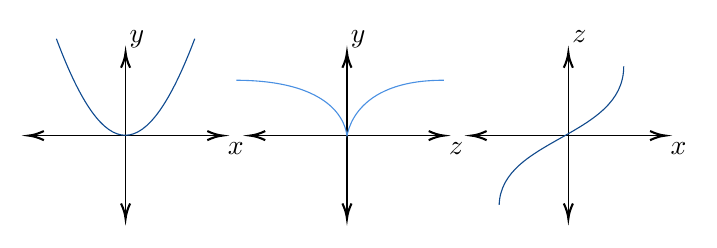
\begin{tikzpicture}[x=0.5pt,y=0.5pt,yscale=-1,xscale=1]
%uncomment if require: \path (0,300); %set diagram left start at 0, and has height of 300

%Straight Lines [id:da7267278045445169] 
\draw    (90,148) -- (90,32) ;
\draw [shift={(90,30)}, rotate = 90] [color={rgb, 255:red, 0; green, 0; blue, 0 }  ][line width=0.75]    (10.93,-3.29) .. controls (6.95,-1.4) and (3.31,-0.3) .. (0,0) .. controls (3.31,0.3) and (6.95,1.4) .. (10.93,3.29)   ;
\draw [shift={(90,150)}, rotate = 270] [color={rgb, 255:red, 0; green, 0; blue, 0 }  ][line width=0.75]    (10.93,-3.29) .. controls (6.95,-1.4) and (3.31,-0.3) .. (0,0) .. controls (3.31,0.3) and (6.95,1.4) .. (10.93,3.29)   ;
%Straight Lines [id:da5494989490391653] 
\draw    (22,90) -- (158,90) ;
\draw [shift={(160,90)}, rotate = 180] [color={rgb, 255:red, 0; green, 0; blue, 0 }  ][line width=0.75]    (10.93,-3.29) .. controls (6.95,-1.4) and (3.31,-0.3) .. (0,0) .. controls (3.31,0.3) and (6.95,1.4) .. (10.93,3.29)   ;
\draw [shift={(20,90)}, rotate = 0] [color={rgb, 255:red, 0; green, 0; blue, 0 }  ][line width=0.75]    (10.93,-3.29) .. controls (6.95,-1.4) and (3.31,-0.3) .. (0,0) .. controls (3.31,0.3) and (6.95,1.4) .. (10.93,3.29)   ;
%Curve Lines [id:da9655294964349719] 
\draw [color={rgb, 255:red, 14; green, 74; blue, 144 }  ,draw opacity=1 ]   (40,20) .. controls (75,113.75) and (105,112.25) .. (140,20) ;
%Straight Lines [id:da8101498601648814] 
\draw    (250,148) -- (250,32) ;
\draw [shift={(250,30)}, rotate = 90] [color={rgb, 255:red, 0; green, 0; blue, 0 }  ][line width=0.75]    (10.93,-3.29) .. controls (6.95,-1.4) and (3.31,-0.3) .. (0,0) .. controls (3.31,0.3) and (6.95,1.4) .. (10.93,3.29)   ;
\draw [shift={(250,150)}, rotate = 270] [color={rgb, 255:red, 0; green, 0; blue, 0 }  ][line width=0.75]    (10.93,-3.29) .. controls (6.95,-1.4) and (3.31,-0.3) .. (0,0) .. controls (3.31,0.3) and (6.95,1.4) .. (10.93,3.29)   ;
%Straight Lines [id:da19278232946906293] 
\draw    (182,90) -- (318,90) ;
\draw [shift={(320,90)}, rotate = 180] [color={rgb, 255:red, 0; green, 0; blue, 0 }  ][line width=0.75]    (10.93,-3.29) .. controls (6.95,-1.4) and (3.31,-0.3) .. (0,0) .. controls (3.31,0.3) and (6.95,1.4) .. (10.93,3.29)   ;
\draw [shift={(180,90)}, rotate = 0] [color={rgb, 255:red, 0; green, 0; blue, 0 }  ][line width=0.75]    (10.93,-3.29) .. controls (6.95,-1.4) and (3.31,-0.3) .. (0,0) .. controls (3.31,0.3) and (6.95,1.4) .. (10.93,3.29)   ;
%Curve Lines [id:da4766073647632322] 
\draw [color={rgb, 255:red, 74; green, 144; blue, 226 }  ,draw opacity=1 ]   (170,50) .. controls (249,50.25) and (249.5,89.25) .. (250,90) .. controls (250.5,90.75) and (253,49.75) .. (320,50) ;
%Straight Lines [id:da5245639166698847] 
\draw    (410,148) -- (410,32) ;
\draw [shift={(410,30)}, rotate = 90] [color={rgb, 255:red, 0; green, 0; blue, 0 }  ][line width=0.75]    (10.93,-3.29) .. controls (6.95,-1.4) and (3.31,-0.3) .. (0,0) .. controls (3.31,0.3) and (6.95,1.4) .. (10.93,3.29)   ;
\draw [shift={(410,150)}, rotate = 270] [color={rgb, 255:red, 0; green, 0; blue, 0 }  ][line width=0.75]    (10.93,-3.29) .. controls (6.95,-1.4) and (3.31,-0.3) .. (0,0) .. controls (3.31,0.3) and (6.95,1.4) .. (10.93,3.29)   ;
%Straight Lines [id:da2916868101444383] 
\draw    (342,90) -- (478,90) ;
\draw [shift={(480,90)}, rotate = 180] [color={rgb, 255:red, 0; green, 0; blue, 0 }  ][line width=0.75]    (10.93,-3.29) .. controls (6.95,-1.4) and (3.31,-0.3) .. (0,0) .. controls (3.31,0.3) and (6.95,1.4) .. (10.93,3.29)   ;
\draw [shift={(340,90)}, rotate = 0] [color={rgb, 255:red, 0; green, 0; blue, 0 }  ][line width=0.75]    (10.93,-3.29) .. controls (6.95,-1.4) and (3.31,-0.3) .. (0,0) .. controls (3.31,0.3) and (6.95,1.4) .. (10.93,3.29)   ;
%Curve Lines [id:da7278244460911197] 
\draw [color={rgb, 255:red, 17; green, 74; blue, 140 }  ,draw opacity=1 ]   (360,140) .. controls (361.5,91.75) and (450,91.25) .. (450,40) ;

% Text Node
\draw (162,93.4) node [anchor=north west][inner sep=0.75pt]    {$x$};
% Text Node
\draw (91,12.4) node [anchor=north west][inner sep=0.75pt]    {$y$};
% Text Node
\draw (322,93.4) node [anchor=north west][inner sep=0.75pt]    {$z$};
% Text Node
\draw (251,12.4) node [anchor=north west][inner sep=0.75pt]    {$y$};
% Text Node
\draw (482,93.4) node [anchor=north west][inner sep=0.75pt]    {$x$};
% Text Node
\draw (411,12.4) node [anchor=north west][inner sep=0.75pt]    {$z$};


\end{tikzpicture}

\end{center}

We set the starting point to be $(0,0,0)$. $\gamma'(t)=(1,2t,3t^2)$. $S(t)=\int_0^t\sqrt{1+4u^2+9u^4}du$


\subsection{Example - Catenary}
A catenary is basically the curved formed by hanging uniform cable.

\begin{center}
    

\tikzset{every picture/.style={line width=0.75pt}} %set default line width to 0.75pt        

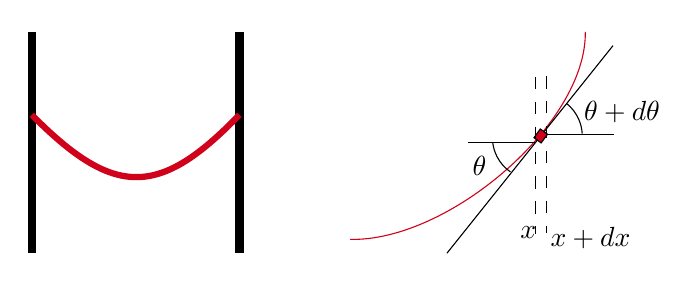
\begin{tikzpicture}[x=0.5pt,y=0.5pt,yscale=-1,xscale=1]
%uncomment if require: \path (0,300); %set diagram left start at 0, and has height of 300

%Straight Lines [id:da46061281192853654] 
\draw [line width=3]    (40,30) -- (40,190) ;
%Straight Lines [id:da184976157035888] 
\draw [line width=3]    (190,30) -- (190,190) ;
%Curve Lines [id:da17626087817705172] 
\draw [color={rgb, 255:red, 208; green, 2; blue, 27 }  ,draw opacity=1 ][line width=2.25]    (40,90) .. controls (99.67,150.33) and (132.33,149.67) .. (190,90) ;
%Curve Lines [id:da5250705726894731] 
\draw [color={rgb, 255:red, 208; green, 2; blue, 27 }  ,draw opacity=1 ]   (270,180) .. controls (341,181.67) and (441,96.33) .. (440,30) ;
%Straight Lines [id:da3839605424088759] 
\draw    (340,190) -- (460,40) ;
%Shape: Rectangle [id:dp09650817368086184] 
\draw  [fill={rgb, 255:red, 208; green, 2; blue, 27 }  ,fill opacity=1 ] (402.89,106.53) -- (407.47,100.23) -- (412.67,104) -- (408.09,110.3) -- cycle ;
%Straight Lines [id:da9571372626114548] 
\draw    (412.67,104) -- (461,104) ;
%Straight Lines [id:da5894329132466996] 
\draw    (355.33,110) -- (403.67,110) ;
%Shape: Arc [id:dp22589905602526306] 
\draw  [draw opacity=0] (426.46,81.78) .. controls (430.22,84.77) and (433.31,88.69) .. (435.34,93.41) .. controls (436.76,96.72) and (437.54,100.14) .. (437.74,103.55) -- (407.78,105.26) -- cycle ; \draw   (426.46,81.78) .. controls (430.22,84.77) and (433.31,88.69) .. (435.34,93.41) .. controls (436.76,96.72) and (437.54,100.14) .. (437.74,103.55) ;  
%Shape: Arc [id:dp9187021553280389] 
\draw  [draw opacity=0] (385.9,131.25) .. controls (381.94,128.54) and (378.59,124.84) .. (376.23,120.28) .. controls (374.58,117.08) and (373.56,113.71) .. (373.13,110.33) -- (402.89,106.53) -- cycle ; \draw   (385.9,131.25) .. controls (381.94,128.54) and (378.59,124.84) .. (376.23,120.28) .. controls (374.58,117.08) and (373.56,113.71) .. (373.13,110.33) ;  
%Straight Lines [id:da7278492168354621] 
\draw  [dash pattern={on 4.5pt off 4.5pt}]  (403.75,62.5) -- (403.75,175.88) ;
%Straight Lines [id:da2272897388146119] 
\draw  [dash pattern={on 4.5pt off 4.5pt}]  (411.75,62) -- (411.75,175.38) ;

% Text Node
\draw (437.33,78.07) node [anchor=north west][inner sep=0.75pt]    {$\theta +d\theta $};
% Text Node
\draw (356.67,118.07) node [anchor=north west][inner sep=0.75pt]    {$\theta $};
% Text Node
\draw (391.25,169.15) node [anchor=north west][inner sep=0.75pt]    {$x$};
% Text Node
\draw (413,169.15) node [anchor=north west][inner sep=0.75pt]    {$x+dx$};


\end{tikzpicture}\\
    a) The general shape. The thick red line denotes the hanging cable. b) Analysis using a unit element(shown as thick red box)
\end{center}
Let the equation be given by $y=f(x)$. Then we note the following:
\begin{enumerate}
    \item $f'(x)=\tan(\theta)$
    \item $T(x)\cos(\theta)=T(x+\Delta x)\cos(\theta+\Delta\theta)$
    \item $T(x)\sin(\theta)+g\delta\Delta S=T(x+\Delta x)\sin(\theta+\Delta\theta)$
\end{enumerate}
In the equations above, $T(x)$ is the tension at $(x,f(x))$, $\delta$ is the mass per unit length and $\Delta S$ is the length of the unit element. From equation 1 and 2 we get:
$$\frac{T(x)}{\sqrt{1+[f'(x)]^2}}=T_0(constant)$$
Put this in 3 to get:
\begin{align*}
    &T(x)\frac{\sin(\theta+\Delta \theta)}{\cos(\theta+\Delta \theta)}\cos(\theta)-T(x)\sin(\theta)=g\delta\Delta S\\
    \Rightarrow&T(x)[\tan(\theta+\Delta\theta)-\tan(\theta)]=g\delta\Delta S\sec(\theta)\\
    \Rightarrow&T(x)\lim_{\Delta x\to0}\frac{\tan(\theta+\Delta \theta)-\tan(\theta)}{\Delta x}=g\delta\sec(\theta)\lim_{\Delta x\to 0}\frac{\Delta S}{\Delta x}\\
    \Rightarrow& T(x)f''(x)=g\delta\sec(\theta)\sqrt{1+[f'(x)]^2}\\
    \Rightarrow&f''(x)=\frac{g\delta}{T(x)\cos(\theta)}\sqrt{1+[f'(x)]^2}\\
    \Rightarrow&f''(x)=c\sqrt{1+[f'(x)]^2}
\end{align*}
Where $c=\frac{g\delta}{T_0}$ is a constant. Now we solve this equation(preferebly with the help of wolfram alpha) to get:
$$f(x)=\frac{\cosh cx}{c}$$


\section{Bending of a curve: Curvature}
\begin{definition}[Curvature] Let $\gamma$ be a regular curve in $\mathbb R^n$. Let $\Delta\theta$ and $\Delta S$ be as shown below.
\begin{center}
    

\tikzset{every picture/.style={line width=0.75pt}} %set default line width to 0.75pt        

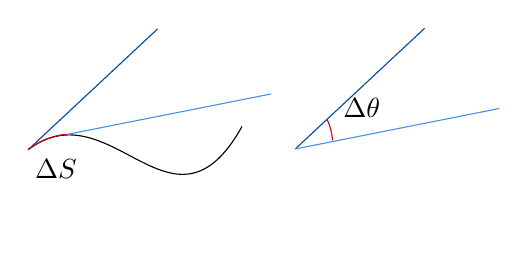
\begin{tikzpicture}[x=0.75pt,y=0.75pt,yscale=-1,xscale=1]
%uncomment if require: \path (0,300); %set diagram left start at 0, and has height of 300

%Curve Lines [id:da9830795993367285] 
\draw    (31,120) .. controls (71,90) and (100.67,168.5) .. (134,108.83) ;
%Straight Lines [id:da32600501780901125] 
\draw [color={rgb, 255:red, 7; green, 72; blue, 147 }  ,draw opacity=1 ]   (31,120) -- (93.33,61.83) ;
%Straight Lines [id:da6697177720117218] 
\draw [color={rgb, 255:red, 74; green, 144; blue, 226 }  ,draw opacity=1 ]   (49.67,112.67) -- (148,93.17) ;
%Curve Lines [id:da8440040891986524] 
\draw [color={rgb, 255:red, 208; green, 2; blue, 27 }  ,draw opacity=1 ]   (31,120) .. controls (36.75,115.13) and (45.25,112.63) .. (49.67,112.67) ;
%Straight Lines [id:da7136675888603832] 
\draw [color={rgb, 255:red, 7; green, 72; blue, 147 }  ,draw opacity=1 ]   (159.67,119.67) -- (222,61.5) ;
%Straight Lines [id:da48210437719433596] 
\draw [color={rgb, 255:red, 74; green, 144; blue, 226 }  ,draw opacity=1 ]   (159.67,119.67) -- (258,100.17) ;
%Shape: Arc [id:dp2406064755275249] 
\draw  [draw opacity=0] (174.94,105.3) .. controls (176.41,108.45) and (177.35,111.89) .. (177.65,115.51) -- (147.75,118) -- cycle ; \draw  [color={rgb, 255:red, 208; green, 2; blue, 27 }  ,draw opacity=1 ] (174.94,105.3) .. controls (176.41,108.45) and (177.35,111.89) .. (177.65,115.51) ;  

% Text Node
\draw (33,123.4) node [anchor=north west][inner sep=0.75pt]    {$\Delta S$};
% Text Node
\draw (181.55,93.95) node [anchor=north west][inner sep=0.75pt]    {$\Delta \theta $};


\end{tikzpicture}

\end{center}
Then the curvature is defined to be rate of change of the tangent vector with curve length or
$$\kappa(t)=\lim_{\Delta t\to0}\frac{\Delta \theta}{\Delta s}$$
\end{definition}
For a unit speed curve, $||\gamma'(S)||=1$. We have the following diagram:
\begin{center}
    

\tikzset{every picture/.style={line width=0.75pt}} %set default line width to 0.75pt        

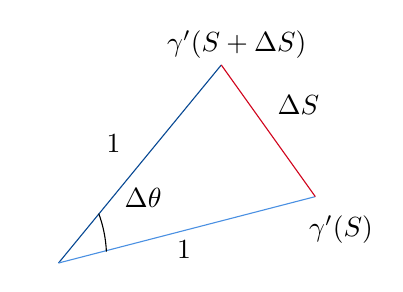
\begin{tikzpicture}[x=0.75pt,y=0.75pt,yscale=-1,xscale=1]
%uncomment if require: \path (0,300); %set diagram left start at 0, and has height of 300

%Straight Lines [id:da7136675888603832] 
\draw [color={rgb, 255:red, 7; green, 72; blue, 147 }  ,draw opacity=1 ]   (72.09,115.72) -- (150.51,20.3) ;
%Straight Lines [id:da48210437719433596] 
\draw [color={rgb, 255:red, 74; green, 144; blue, 226 }  ,draw opacity=1 ]   (72.09,115.72) -- (195.8,83.73) ;
%Shape: Arc [id:dp2406064755275249] 
\draw  [draw opacity=0] (91.46,91.91) .. controls (93.55,97.51) and (94.85,103.71) .. (95.16,110.25) -- (57.49,113.39) -- cycle ; \draw  [color={rgb, 255:red, 0; green, 0; blue, 0 }  ,draw opacity=1 ] (91.46,91.91) .. controls (93.55,97.51) and (94.85,103.71) .. (95.16,110.25) ;  
%Straight Lines [id:da4722233081523145] 
\draw [color={rgb, 255:red, 208; green, 2; blue, 27 }  ,draw opacity=1 ]   (150.51,20.3) -- (195.8,83.73) ;

% Text Node
\draw (102.71,78.4) node [anchor=north west][inner sep=0.75pt]    {$\Delta \theta $};
% Text Node
\draw (191.6,91.8) node [anchor=north west][inner sep=0.75pt]    {$\gamma '( S)$};
% Text Node
\draw (123.2,2.6) node [anchor=north west][inner sep=0.75pt]    {$\gamma '( S+\Delta S)$};
% Text Node
\draw (176.4,33.6) node [anchor=north west][inner sep=0.75pt]    {$\Delta S$};
% Text Node
\draw (128,103.8) node [anchor=north west][inner sep=0.75pt]    {$1$};
% Text Node
\draw (94,52.6) node [anchor=north west][inner sep=0.75pt]    {$1$};


\end{tikzpicture}

\end{center}
We note:
\begin{align*}
    &||\gamma'(S+\Delta S)-\gamma'(S)||={2\sin\left(\frac{\theta}{2}\right)}\\
    \Rightarrow&\frac{\Delta\theta}{\Delta S}=\frac{\Delta\theta/2}{\sin\left(\frac{\theta}{2}\right)}\frac{||\gamma'(S+\Delta S)-\gamma'(S)||}{\Delta S}=|\gamma''(S)|
\end{align*}
We immidietly notice for curvature to be defined we eed:
\begin{enumerate}
    \item $\gamma$ to be Regular
    \item $\gamma''$ to be defined 
\end{enumerate}
\textit{Notation:}If $\gamma$ is unit speed then we use $s$ as the parameter.
\subsection{Examples}
\begin{enumerate}
    \item For a straightline given by $\gamma(t)=\vec{a}+\vec{p}t$, Curvature is 0
    \item For a circle of radius $r$ given by $\gamma(t)=(x_0,y_0)+\left(r\cos\left(\frac{t}{r}\right),r\sin\left(\frac{t}{r}\right)\right)$, curvature=$||\gamma''||=\frac{1}{r}$
\end{enumerate}
\subsection{Calculation of curvature for space curves}
Let $\gamma$ be a regular $C^3$ curve. The curvature is given by:
$$\kappa(t):=\frac{||\gamma'(t)\times\gamma''(t)||}{||\gamma'(t)||^3}$$
\subsection{Remarks}
\begin{enumerate}
    \item If $\gamma$ lies on an unit sphere, with $||\gamma''||=1$ Then $<\gamma(t),\gamma(t)>=1\Rightarrow <\gamma(t),\gamma'(t)>=0$. Therefore, $\kappa(t)=1$. In this case, $\gamma''(t)$ essentially measures the rate of change of dirction of the curve.  
\end{enumerate}
























\part{The Riemann Uniformization Theorem}















\part{End Notes}
\chapter{Appendix}
\section{Some specific curves taught in class}
\subsection{Parabola}




\section{Differentiability of curves}
\begin{definition}[Differentiable function]
A continuous function $f:(a,b)\to\mathbb R$(\textit{Note:} $a,b$ might be $\pm \infty$, in which case the function is defined on whole of $\mathbb R$) is called differentiable or of type $c^1$ if $$f'(x)=\lim_{h\to 0}\frac{f(x+h)-f(x)}{h}$$
exists and is continuous.
\end{definition}
In a similar way, we can define $C^2,C^3$ and  $C^k$ by differentiating $f$ $2,3,k$ times respectively. We call a function ``\textit{smooth}'' if the function is $C^k$ for any $k\in\mathbb N$.\\
\textbf{Examples}
\begin{enumerate}
    \item $f(x)=|x|$: This is a $C^0$ function as $f$ is not differentiable at 0.
    \item $$f(x)=\begin{cases}x^2\sin\left(\frac{1}{x}\right)\quad&x\ne0\\
    0\quad&x=0
    \end{cases}$$
    $f'$ exists but is not continuous. So $f'$ is not continuous. 
\end{enumerate}
\section{Differentiation (Multivariable)}
\begin{definition}[Differentiable multivariable function]
A function $f:(a,b)\to\mathbb R$ is of class $C^k$ if every $\pi_i\circ f(x)$ is $C^k$ where $\pi_i$ is projection to the $i^{th}$ coordinate.
\end{definition}
\textbf{Notation:} We define $$\nabla_vf(p)=\lim_{t\to 0}\frac{f(p+tv)-f(p)}{t} $$\\
For $C^1$ functions let $v=v_1+v_2$. Then:
\begin{align*}
    \nabla_vf(p)-\nabla_{v_1}f(p)&=\lim_{t\to0}\frac{f(p+tv_1+tv_2)-f(p+tv_1)}{t}\\
    &=\lim_{t\to0}\nabla_{v_2}f(p+tv_1)=\nabla_{v_2}f(p) 
\end{align*}
\begin{align*}
    \nabla_{kv}f(p)&=\lim_{t\to0}\frac{f(p+tkv)-f(p)}{t}\\
    &=k\lim_{t\to0}\frac{f(p+tkv)-f(p)}{kt}\\
    &=k\nabla_vf(p)    
\end{align*}
If $v=\sum_{i=1}^nc_ie_i$, then we can apply the above formula repeatedly to get   $\nabla_vf(p)=\sum_{i=1}^nc_i\nabla_{e_i}f(p)$.
\begin{definition}[Differentiation of multivariable function]
A function $\mathbb R^n\to\mathbb R^m$ is differntiable at $a$ if there exists a linear map $L_a:\mathbb R^n\to\mathbb R^m$ such that
$$f(a+v)-f(a)-L_a(v)=E_a(v)||v||$$
where $\lim_{v\to 0}E_a(v)=0$.
\end{definition}
A function $f$ is called differntiable if such a linear map exists and $D_f(a)=L_a$. We can define a map $\Tilde{D_f}:\mathbb R^n\times\mathbb R^m\to\mathbb R^m,\Tilde{D_f}(a,v)=L_av$. This map is studied in differential geometry. 
%%Need to prove D_f is cts iff \tilde D_f is cts.
A nice condition is if all the $k^{th}$ derivative $\frac{\partial^k}{\partial x_i^{k_i}}f,\sum k_i=k$ exits and is continuous then $f$ is $C^k$ continuous. 
\section{Homeomorphism, Diffeomorphism and invariance of domain}
\begin{definition}[Diffeomorphism]
Let $U\in\mathbb R^n$ and $V\in\mathbb R^m$ be open sets of $\mathbb R^n$ and $\mathbb R^m$ repectively. A map $f:U\to V$ is a diffeomorphism if $f$ is $C^\infty$ and if $f$ has a smooth inverse.
\end{definition}
If we consider homeomorphism between $U,V$ then it is required that $m=n$. This proof requires techniques of algebric topology and is not discussed here.This is known as invariance of domain. But if we consider difeomorphisms, then we can prove $m=n$.
\begin{lemma}
Let $f:\mathbb R^l\to\mathbb R^m$ and $g:\mathbb R^m\to\mathbb R^n$ are smooth function then $f\circ g$ is smooth. 
\end{lemma}
\textbf{Notation: }We shall look at a nice way to write the differentiation operator. We say
$$Df(a,v)=D_f(a)v$$
For example, we shall write the chain rule as
$$D(g\circ f)(\overrightarrow{a},\overrightarrow{v})=Dg(f(\overrightarrow{a}),Df(\overrightarrow{a},\overrightarrow{v}))$$
\begin{corollary}
If there exists a difeeomorphism between $U\in\mathbb R^n$ and $V\in\mathbb R^m$ then $m=n$.
\end{corollary}
\begin{proof}
Without loss of generality, let $m\geq n$. Let $f:U\to V$ be the diffeomorphism and let $g$ be it's inverse. Then $D(f\circ g)(\overrightarrow{a},\cdot)=D(Id_{m\times m})(\overrightarrow{a},\cdot)=Id_{m\times m}$. This follows because differentiation of a linear map $T$ is $T$ itself. But we also have
$$D(f\circ g)(\overrightarrow{a},\cdot)=Dg(f(\overrightarrow{a}),Df(\overrightarrow{a},\cdot))$$
Let $D_g(f(a))=L_{m}^n$ and $D_f(a)=L_{n}^m$. Therefore:
$$D(f\circ g)(\overrightarrow{a},v)=L_{n}^mL_m^nv$$
Now we use the rank nullity theorem. 
\begin{align*}
    dim(null(L_{m}^n))&=dim \mathbb{R}^m-dim(range(L_{m}^n))\\
    &\geq m-dim(\mathbb R^n)=m-n
\end{align*}
Now if $dim(null(L_{m}^n))\ne 0$ then we can get $v\ne 0$ such that $L_{n}^mL_m^nv=L_{n}^m0=0$. But this shouldn't happen as $L_{n}^mL_m^nv=Id_{m\times m}v=v$. So we need $m-n=0\Rightarrow m=n$.
\end{proof}
\textit{Note:} Our instructor gave a slight variation of the proof: he mentioned $L_{n}^mL_m^nv$ and $L_m^nvL_{n}^m$ can't be both invertible if $m\ne n$. I felt what he said was trivial but still need to be written out.





\end{document}
